% =====================================================================
% ARTI5001 Assignment 3 — Report
% Single-speaker TTS on LJSpeech: flow-matching vs regression decoders
%
% Overleaf: New Project > Upload Project > zip of this report/ folder. Compiler: pdfLaTeX.
% Bibliography: references.bib, Harvard (author-year) via natbib + agsm.
% LIMIT: 12 A4 pages INCLUDING references. Page budget per section is given in each header comment.
%
% \ph{...}   = placeholder (red box), so nothing unfinished slips through. Search for "\ph{" before submitting.
% Numbers already filled in come from the notebook (notebook/A3_final.ipynb, section numbers given as "nb §x.y.z").
% =====================================================================
\documentclass[11pt,a4paper]{article}
\usepackage[margin=2.2cm]{geometry}
\usepackage[T1]{fontenc}
\usepackage{lmodern,microtype}
\usepackage{graphicx,booktabs,tabularx,multirow,xcolor,enumitem,caption,subcaption}
\usepackage{amsmath,amssymb}
\usepackage{tikz}
\usetikzlibrary{positioning,arrows.meta,fit,backgrounds}
\usepackage[round]{natbib}          % Harvard (author-year) citations: \citet{} = Author (Year), \citep{} = (Author, Year)
\usepackage[hidelinks]{hyperref}
\setlist{nosep}
\captionsetup{font=small,labelfont=bf}

\newcommand{\ph}[1]{\colorbox{red!12}{\textcolor{red!70!black}{\small\textsf{[#1]}}}}
\newcommand{\expA}{\texttt{expA}}
\newcommand{\expB}{\texttt{expB}}
\newcommand{\expC}{\texttt{expC}}
\newcommand{\expD}{\texttt{expD}}

% =====================================================================
% TITLE PAGE (group details)
% =====================================================================
\begin{document}
\begin{titlepage}
\centering
\vspace*{3cm}
{\LARGE\bfseries Text-to-Speech on LJSpeech:\\[6pt]
Does a Generative Decoder Beat Regression?\par}
\vspace{8mm}
{\large A controlled comparison of flow-matching and regression mel decoders\\ in a from-scratch acoustic model\par}
\vspace{2cm}
{\large ARTI5001 Generative Artificial Intelligence --- Assignment 3\par}
\vspace{1cm}
{\large Group 44\par}
\vspace{5mm}
{\large
\begin{tabular}{ll}
Varuna Lingam Pavalla Maharudramurthy & a1940373 \\
Romeo Lama & a1985312 \\
En Li & a1993209 \\
\end{tabular}\par}
\vfill
{\large Adelaide University \quad\textbullet\quad \ph{DD} November 2026\par}
\end{titlepage}

% =====================================================================
% EXECUTIVE SUMMARY  (non-technical, <= 1 page)
% =====================================================================
\section*{Executive Summary}
% Write for a manager, not an engineer: no jargon (no "mel", "ODE", "MAS"). Cover problem, system, result, value,
% feasibility/scaling, recommendation. Fill in AFTER the results are in.

\noindent\textbf{The problem.} Turning written text into natural-sounding speech (text-to-speech) underpins screen readers, audiobooks, voice assistants and announcement systems. Good systems usually need large datasets and expensive computers. We asked how good a voice a small team can build \emph{from scratch} on one laptop, and which design choice matters most.

\noindent\textbf{What we built.} A working system that takes any English sentence and produces a recording in the voice of a single speaker. It was trained on about 5.5 hours of one speaker's audiobook recordings. \ph{one sentence: what it handles well, e.g. numbers, abbreviations, punctuation}

\noindent\textbf{What we compared.} The final ``speaking'' step of the system can be built in two ways. One predicts the sound directly in a single fast step. The other generates it gradually over several steps, which costs more time. We built both, each in a large and a small size, and gave all four versions identical data and training time.

\noindent\textbf{What we found.} \ph{headline result in everyday terms, e.g. ``the gradual version was clearly more natural and X\% more intelligible to an automatic listener, while still producing speech N times faster than real time''}

\noindent\textbf{Practical value and cost.} \ph{e.g. one hour of speech generated in N minutes on a laptop; no specialised hardware needed at run time}

\noindent\textbf{Feasibility and scaling.} \ph{what a production version would need: more data, a GPU for training, CPU is enough for serving, \ldots}

\noindent\textbf{Recommendation.} \ph{which version to use and why, in one sentence}
\newpage

% =====================================================================
% 1. INTRODUCTION AND PROBLEM FRAMING  (~0.75 page)
% =====================================================================
\section{Introduction and Problem Framing}
Modern neural text-to-speech (TTS) systems split the task into stages \citep{shen2018tacotron2,ren2021fastspeech2}. A text front-end converts text into phonemes. An \emph{acoustic model} predicts a mel spectrogram from the phonemes. A \emph{vocoder} converts the mel spectrogram into a waveform. The acoustic model decides \emph{what} is said, for \emph{how long} and with \emph{which} spectral detail, so it is where most design decisions sit.

A central choice inside the acoustic model is how the final mel decoder is trained. \emph{Regression} decoders \citep{ren2021fastspeech2} predict the mel directly with an $L_1$/$L_2$ loss. They are fast and simple, but they are known to produce over-smoothed spectra, because they learn the average of all plausible renditions. \emph{Generative} decoders, such as diffusion \citep{popov2021gradtts} or conditional flow matching \citep{mehta2024matcha}, instead learn a distribution and sample from it. The cost is several network evaluations per utterance.

\noindent\textbf{Aim.} To build a complete, reproducible TTS pipeline on LJSpeech \citep{ito2017ljspeech} with an acoustic model implemented and trained from scratch, and to measure, under controlled conditions, how the decoder objective and the decoder depth affect intelligibility, quality and speed.

\noindent\textbf{Scope.}
\begin{itemize}
  \item Single speaker (LJSpeech) and English only.
  \item A 3{,}000-utterance training subset (about 5.5\,h) and an equal budget of 300 epochs per experiment, on one Apple M4 laptop.
  \item A pretrained, frozen HiFi-GAN vocoder \citep{kong2020hifigan}.
  \item Out of scope: multi-speaker training, emotion and style control, and training a vocoder.
\end{itemize}

\noindent\textbf{Research questions.}
\textbf{RQ1:} Does a flow-matching decoder produce more natural and intelligible speech than a regression decoder of the same size, and at what inference cost?
\textbf{RQ2:} How much does decoder depth (8 vs 4 residual blocks) matter, and does the answer depend on the objective?

\noindent\textbf{Contributions.}
\begin{itemize}
  \item A reproducible LJSpeech pipeline: integrity checks, a justified text and audio front-end, and a fixed 80/10/10 split (seed 42, MD5-fingerprinted).
  \item A Matcha-style acoustic model written from scratch, with two interchangeable decoders that share one backbone.
  \item A $2\times2$ factorial experiment in which every compared pair differs in exactly one variable (checked in code).
  \item A multi-metric evaluation (RTF, latency, ASR-based WER/CER, \ph{MCD / UTMOS}), plus listening evidence and an error analysis.
\end{itemize}

% =====================================================================
% 2. BACKGROUND (short, ~0.5 page) — optional but helps "justification"; merge into §1 if space is tight
% =====================================================================
\section{Background}
\textbf{Acoustic models.} Autoregressive models such as Tacotron~2 \citep{shen2018tacotron2} generate one frame at a time with attention. They are natural-sounding but slow, and they are prone to skipping or repeating words. Non-autoregressive models such as FastSpeech~2 \citep{ren2021fastspeech2} predict a duration for every phoneme and then all frames in parallel. Glow-TTS \citep{kim2020glowtts} removed the need for an external aligner with \emph{Monotonic Alignment Search} (MAS), which learns the alignment jointly with the model.

\textbf{Generative decoders.} Grad-TTS \citep{popov2021gradtts} adds a diffusion decoder conditioned on a frame-level prior. It is high quality, but needs tens to hundreds of steps. Matcha-TTS \citep{mehta2024matcha} replaces diffusion with optimal-transport conditional flow matching \citep{lipman2023flowmatching}. This learns straight noise-to-data paths, so about 10 steps suffice.

\textbf{End-to-end models.} VITS \citep{kim2021vits} maps text directly to a waveform with a VAE and adversarial training. It gives high quality, but is harder to train and to analyse.

\textbf{Vocoders.} HiFi-GAN \citep{kong2020hifigan} is a GAN vocoder that is both fast and high quality. It is the standard companion of mel-based acoustic models.

\noindent Our system follows the Matcha-TTS and Glow-TTS family, simplified. The decoder objective, the main design question in this family, is our controlled variable.

% =====================================================================
% 3. SYSTEM DESIGN (with diagram) AND JUSTIFICATION  (~2 pages)
% =====================================================================
\section{System Design}\label{sec:design}
% HD: clear diagram + role of EACH module + choices justified by linking constraints -> decisions -> goals.
% If you draw the diagram in Mermaid/draw.io instead, export to figures/pipeline.pdf and replace the tikzpicture with
%   \includegraphics[width=\linewidth]{figures/pipeline.pdf}

\begin{figure}[t]
\centering
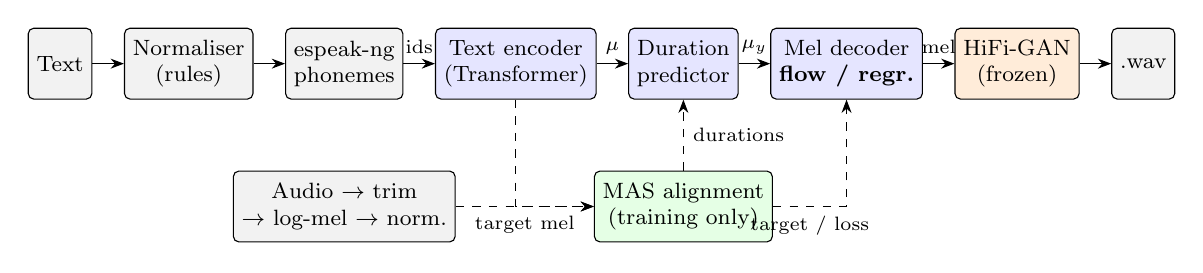
\begin{tikzpicture}[node distance=3.5mm and 4mm, >=Stealth,
  box/.style={draw, rounded corners=2pt, align=center, minimum height=9mm, font=\footnotesize, inner sep=3pt},
  rule/.style={box, fill=gray!10},
  ours/.style={box, fill=blue!10},
  pre/.style={box, fill=orange!15},
  lab/.style={font=\scriptsize, midway, above}]
  % inference path
  \node[rule] (txt) {Text};
  \node[rule, right=of txt] (norm) {Normaliser\\(rules)};
  \node[rule, right=of norm] (g2p) {espeak-ng\\phonemes};
  \node[ours, right=of g2p] (enc) {Text encoder\\(Transformer)};
  \node[ours, right=of enc] (dur) {Duration\\predictor};
  \node[ours, right=of dur] (dec) {Mel decoder\\\textbf{flow / regr.}};
  \node[pre, right=of dec] (voc) {HiFi-GAN\\(frozen)};
  \node[rule, right=of voc] (wav) {.wav};
  \draw[->] (txt) -- (norm); \draw[->] (norm) -- (g2p); \draw[->] (g2p) -- node[lab]{ids} (enc);
  \draw[->] (enc) -- node[lab]{$\mu$} (dur); \draw[->] (dur) -- node[lab]{$\mu_y$} (dec);
  \draw[->] (dec) -- node[lab]{mel} (voc); \draw[->] (voc) -- (wav);
  % training-only path
  \node[rule, below=9mm of g2p] (audio) {Audio $\rightarrow$ trim\\$\rightarrow$ log-mel $\rightarrow$ norm.};
  \node[ours, below=9mm of dur, fill=green!10] (mas) {MAS alignment\\(training only)};
  \draw[->, dashed] (audio) -- node[lab, below]{target mel} (mas);
  \draw[->, dashed] (enc.south) |- (mas.west);
  \draw[->, dashed] (mas) -- node[font=\scriptsize, right]{durations} (dur.south);
  \draw[->, dashed] (mas.east) -| node[font=\scriptsize, pos=0.25, below]{target / loss} (dec.south);
\end{tikzpicture}
\caption{The pipeline. Solid arrows show inference, dashed arrows show training only. Blue modules are implemented and trained from scratch by us, orange is pretrained and frozen, and grey is rule-based. Only the \textbf{mel decoder} differs between experiments.}
\label{fig:pipeline}
\end{figure}

\subsection{Modules}
Table~\ref{tab:modules} lists every module, its role and its tensor interface. Parameter counts are for the baseline \expA.

\begin{table}[h]
\centering\small
\caption{Modules, their roles and their interfaces ($L$ = phonemes, $T$ = mel frames of 11.6\,ms).}
\label{tab:modules}
\begin{tabularx}{\linewidth}{@{}l>{\raggedright\arraybackslash}Xll@{}}
\toprule
Module & Role & Input $\rightarrow$ Output & Params \\ \midrule
Text normaliser & Spells out abbreviations, numbers, money and times; ASCII and lower case; keeps prosodic punctuation & string $\rightarrow$ string & -- \\
Phonemiser & espeak-ng IPA with stress marks \citep{bernard2021phonemizer}; 55-symbol vocabulary from the training split & string $\rightarrow$ ids $[L]$ & -- \\
Text encoder & Embedding, 6-layer Transformer \citep{vaswani2017attention} ($d{=}192$), and a projection to a per-phoneme mel prior $\mu$ & $[L] \rightarrow [L{\times}80]$ & 2.89\,M \\
MAS (training only) & Finds the most likely monotonic phoneme-to-frame alignment, giving target durations \citep{kim2020glowtts} & $\mu$, mel $\rightarrow$ durations $[L]$ & -- \\
Duration predictor & 3 conv layers predicting log-durations; at inference, expands $\mu$ to frame level $\mu_y$ & $[L{\times}192] \rightarrow [L]$ & 0.34\,M \\
Mel decoder & Refines $\mu_y$ into the final mel with residual conv blocks (256 ch.); \textbf{flow matching or regression; 8 or 4 blocks} & $[80{\times}T] \rightarrow [80{\times}T]$ & 4.27\,M \\
Vocoder & HiFi-GAN V1 trained on LJSpeech \citep{kong2020hifigan}, frozen & $[80{\times}T] \rightarrow [256T]$ samples & 13.94\,M \\ \bottomrule
\end{tabularx}
\end{table}

\noindent\textbf{Training objective.} The total loss is the sum of three terms: the duration loss (MSE on log-durations from MAS), the prior loss (Gaussian negative log-likelihood of the target mel under $\mu_y$) and the decoder loss.
For the \textbf{flow-matching} decoder \citep{lipman2023flowmatching,mehta2024matcha}, we sample $x_0\!\sim\!\mathcal N(0,I)$ and $t\!\sim\!U[0,1]$, set $x_t=(1-(1-\sigma_{\min})t)\,x_0+t\,x_1$, and regress the network's velocity $v_\theta(x_t,\mu_y,t)$ onto $u=x_1-(1-\sigma_{\min})x_0$. At inference it integrates $v_\theta$ from noise (temperature 0.667) with 10 Euler steps.
The \textbf{regression} decoder uses the same backbone without the time input, and minimises the masked $L_1$ distance between its single-pass output and $x_1$.

\subsection{Design Justification}
Table~\ref{tab:justify} links each constraint to the decision it led to and the evidence behind it. The full list of decisions, with alternatives, is in the notebook (nb~§1.2.1).

\begin{table}[h]
\centering\small
\caption{Constraints $\rightarrow$ decisions $\rightarrow$ consequences.}
\label{tab:justify}
\begin{tabularx}{\linewidth}{@{}>{\raggedright\arraybackslash}p{2.9cm}>{\raggedright\arraybackslash}X>{\raggedright\arraybackslash}X@{}}
\toprule
Constraint / goal & Decision & Consequence / evidence \\ \midrule
Build the acoustic model ourselves; one laptop GPU (Apple M4, 16\,GB) & Compact Matcha-style model (5--7.5\,M params) with a 1-D conv decoder instead of Matcha's U-Net & About 54\,s per epoch for \expA; 300 epochs in about 4.7\,h \\
No external aligner available; avoid attention failures & MAS \citep{kim2020glowtts} with a duration predictor & Alignment is monotonic by construction, so no skipped or repeated words; fully parallel inference \\
English spelling is ambiguous; small data & IPA phonemes from espeak-ng, stress kept & The model learns pronunciation, not spelling rules; no out-of-vocabulary symbols in val/test (nb §1.1.9.3) \\
Training a vocoder takes days & Pretrained HiFi-GAN V1; our mel settings \emph{match} it exactly (1024/256/1024, 80 bands, 0--8\,kHz) & High-fidelity waveforms from the first epoch; one vocoder shared by all runs keeps the comparison fair \\
Flow matching starts from $\mathcal N(0,I)$ & Global mel normalisation with training-subset mean/std ($-5.50$ / $2.06$) & Targets on the noise scale; no leakage from val/test \\
Goal: real-time synthesis & Non-autoregressive model; 10 ODE steps rather than diffusion's 50--1000 & \ph{RTF from Table~\ref{tab:results}} \\ \bottomrule
\end{tabularx}
\end{table}

\noindent\textbf{Alternatives rejected.}
\begin{itemize}
  \item \emph{Fine-tuning a pretrained VITS:} a from-scratch acoustic model makes the decoder a clean controlled variable and keeps every design decision ours.
  \item \emph{Tacotron~2 with attention:} slower and less robust on 5\,h of data.
  \item \emph{A diffusion decoder:} it needs many more sampling steps for similar quality \citep{mehta2024matcha}.
  \item \emph{Griffin--Lim instead of a neural vocoder:} it gives audibly robotic output.
\end{itemize}

% =====================================================================
% 4. EXPERIMENTAL DESIGN  (~1.5 pages)
% =====================================================================
\section{Experimental Design}\label{sec:expdesign}
% HD: >=2 controlled experiments with a clear comparison goal; protocol explicit and CONSISTENT WITH THE CODE.

\subsection{Data Protocol}
\textbf{Dataset.} We use LJSpeech~1.1 \citep{ito2017ljspeech}: 13{,}100 clips (23.92\,h) of one female speaker, 22{,}050\,Hz mono 16-bit. All files were checked for format, readability and a matching transcript (nb §1.1.6). The metadata must be parsed with \texttt{QUOTE\_NONE}; otherwise quote characters swallow the delimiter and 16 transcripts appear empty.

\noindent\textbf{Split.} 80/10/10 (10{,}480 / 1{,}310 / 1{,}310 clips). The IDs are sorted and shuffled with \texttt{numpy} seed 42, and the split's MD5 is \texttt{78fda0eda5bbdcaecb57fd47e9b20610}. Each experiment trains on the same seeded \textbf{3{,}000-utterance subset} of the training split (5.5\,h). A fixed 300-clip subset of validation is scored every epoch. The test split is held out for evaluation.

\noindent\textbf{Preprocessing} (Table~\ref{tab:preproc}). Every choice was driven by a measurement of the raw data (nb §1.1.7).
\begin{table}[h]
\centering\small
\caption{Preprocessing decisions and the evidence for each.}
\label{tab:preproc}
\begin{tabularx}{\linewidth}{@{}l>{\raggedright\arraybackslash}p{4.3cm}>{\raggedright\arraybackslash}X@{}}
\toprule
Step & Choice & Evidence / reason \\ \midrule
Sample rate & keep 22{,}050\,Hz & all files already 22{,}050\,Hz; equal to the vocoder's rate \\
Silence & trim edges, \texttt{top\_db}=40 & leading $\approx$0\,s but trailing $\approx$80\,ms in almost every clip; MAS would otherwise attach it to the last phoneme. Removes 1.2\% of the audio; no clip loses more than half its length \\
Loudness & none & speech RMS spread of only 1.25\,dB across clips \\
Text source & normalised column & raw: 1{,}489 clips with digits; normalised: 0 \\
Abbreviations & expand (\textit{Mr.} $\rightarrow$ \textit{mister}) & still present in 573 normalised transcripts \\
Numbers & spell out (\texttt{num2words}) & needed for arbitrary input at inference \\
Tokens & IPA phonemes, stress marks & 55 symbols; average 105 tokens per clip \\
Mel & 80-band log-mel matching HiFi-GAN; global mean/std from the training subset & vocoder compatibility; no leakage \\ \bottomrule
\end{tabularx}
\end{table}

\subsection{Controlled Variables and Hypotheses}
We use a $2\times2$ factorial design (Table~\ref{tab:settings}). Each comparison changes exactly one variable, and this is asserted in code (nb §1.3.3).
\begin{itemize}
  \item \textbf{Objective} (\expA\ vs \expC, \expB\ vs \expD): flow matching vs regression at equal depth.
  \item \textbf{Depth} (\expA\ vs \expB, \expC\ vs \expD): 8 vs 4 residual blocks with the same objective.
\end{itemize}
\textbf{H1:} regression decoders produce over-smoothed mels, so their speech sounds more muffled and scores worse on quality metrics.
\textbf{H2:} regression is faster at inference: one decoder pass versus ten.
\textbf{H3:} the 4-block decoders are faster with a small quality loss, and depth matters more for flow matching, which must model a whole distribution.

\subsection{Training and Selection Protocol}
\begin{itemize}
  \item \textbf{Shared settings:} Adam (lr $10^{-4}$), batch 32, gradient clipping 1.0 and 300 epochs (93 steps per epoch, 27{,}900 steps in total) for every experiment, seed 42, on an Apple M4 (PyTorch MPS).
  \item \textbf{Validation:} the validation loss is computed every epoch on the same 300 clips with a fixed random seed, so the noisy flow loss is comparable across epochs.
  \item \textbf{Checkpoints:} \texttt{best.ckpt} is the epoch with the lowest validation loss \emph{within} each experiment. Milestone checkpoints are kept at epochs 75, 150, 225 and 300.
  \item \textbf{Comparability:} total losses are not comparable across objectives (velocity MSE vs mel $L_1$). Cross-experiment comparison therefore uses only the evaluation metrics in Section~\ref{sec:results}, plus the duration and prior losses, which come from identical modules.
\end{itemize}

\begin{table}[h]
\centering\small
\caption{Experiment settings. Bold marks the controlled variables; everything else is identical. Training time excludes one 13.6-hour stall caused by the laptop sleeping during \expA.}
\label{tab:settings}
\begin{tabular}{@{}lcccc@{}}
\toprule
 & \expA\ (baseline) & \expB & \expC & \expD \\ \midrule
\textbf{Decoder objective} & \textbf{flow matching} & \textbf{flow matching} & \textbf{regression} & \textbf{regression} \\
\textbf{Decoder blocks} & \textbf{8} & \textbf{4} & \textbf{8} & \textbf{4} \\
Parameters (total / decoder) & 7.50 / 4.27\,M & 5.66 / 2.43\,M & 6.43 / 3.20\,M & 4.85 / 1.62\,M \\
Decoder passes at inference & 10 & 10 & 1 & 1 \\
Data / split / seed & \multicolumn{4}{c}{3{,}000 utts \quad / \quad 80/10/10 \quad / \quad 42} \\
Epochs / batch / lr & \multicolumn{4}{c}{300 \quad / \quad 32 \quad / \quad $10^{-4}$} \\
Best epoch (val. loss) & 281 (1.942) & \ph{} & \ph{} & \ph{} \\
Training time & 4.7\,h & \ph{} & \ph{} & \ph{} \\ \bottomrule
\end{tabular}
\end{table}

% =====================================================================
% 5. RESULTS AND EVALUATION  (~2.5 pages)
% =====================================================================
\section{Results and Evaluation}\label{sec:results}
% HD: metrics reported clearly AND INTERPRETED; audio evidence USED in a reasoned trade-off discussion.

\subsection{Evaluation Protocol}
\begin{itemize}
  \item \textbf{Speed:} RTF = synthesis time $/$ audio duration, and latency per sentence (mean $\pm$ std, after \ph{3} warm-up runs and \ph{N} timed repeats, on \ph{device}). Both are measured for the acoustic model plus vocoder.
  \item \textbf{Intelligibility:} WER and CER of Whisper \citep{radford2022whisper} transcripts of \ph{N} test sentences, against our normalised text. Ground-truth recordings give the upper bound.
  \item \textbf{Quality:} \ph{MCD \citep{kubichek1993mcd} against the test recordings, with DTW, and/or UTMOS predicted MOS}.
  \item \textbf{Listening evidence:} \ph{10+} prompts per experiment (\texttt{wav\_examples/expX\_NN.wav}), including hard cases (numbers, long sentences, questions, names).
\end{itemize}

\subsection{Training Behaviour}
\ph{Figure: training curves (results/figures/1\_3\_training\_curves.png). One or two sentences: all runs converged; validation loss flattened after about epoch 200; duration and prior losses compared across runs.}
% \begin{figure}[h]\centering\includegraphics[width=\linewidth]{figures/1_3_training_curves.png}
% \caption{Training curves. Solid: flow matching; dashed: regression; star: best.ckpt.}\label{fig:curves}\end{figure}

\subsection{Objective Metrics}
\begin{table}[h]
\centering\small
\caption{Objective results on the test set (\ph{N} sentences; device \ph{}). Arrows show the better direction; best values in bold.}
\label{tab:results}
\begin{tabular}{@{}lcccccc@{}}
\toprule
 & RTF $\downarrow$ & Latency (s) $\downarrow$ & WER (\%) $\downarrow$ & CER (\%) $\downarrow$ & \ph{MCD (dB)} $\downarrow$ & \ph{UTMOS} $\uparrow$ \\ \midrule
\expA\ flow, 8 & \ph{} & \ph{} & \ph{} & \ph{} & \ph{} & \ph{} \\
\expB\ flow, 4 & \ph{} & \ph{} & \ph{} & \ph{} & \ph{} & \ph{} \\
\expC\ regr., 8 & \ph{} & \ph{} & \ph{} & \ph{} & \ph{} & \ph{} \\
\expD\ regr., 4 & \ph{} & \ph{} & \ph{} & \ph{} & \ph{} & \ph{} \\ \midrule
Ground truth & -- & -- & \ph{} & \ph{} & 0 & \ph{} \\
Vocoded ground truth & -- & -- & \ph{} & \ph{} & \ph{} & \ph{} \\ \bottomrule
\end{tabular}
\end{table}

\noindent\textbf{RQ1, the objective.} \ph{Interpret A vs C and B vs D. Is the difference larger than the spread between sentences? Does it support H1 and H2?}

\noindent\textbf{RQ2, depth.} \ph{Interpret A vs B and C vs D. Does it support H3? Is there an interaction between objective and depth?}

\noindent\textbf{ODE steps (optional).} \ph{RTF and quality of \expA\ at 2, 4, 10 and 20 steps: where is the knee of the quality--speed curve?}

\subsection{Qualitative Evidence}
\ph{Listening notes tied to specific files, e.g. ``\texttt{expC\_04.wav} sounds muffled and buzzy on vowels, while \texttt{expA\_04.wav} is crisp.'' If possible, give blind A/B preference counts from the group (n = 3 listeners $\times$ 10 prompts).}

\ph{Figure: mel spectrograms of one test sentence (ground truth, \expA, \expC). Regression should show blurred harmonics, which is the visual evidence for H1.}
% \begin{figure}[h]\centering\includegraphics[width=\linewidth]{figures/spec_compare.png}
% \caption{Mel spectrograms of test sentence LJ0XX-XXXX.}\label{fig:spec}\end{figure}

\subsection{Trade-offs}
\ph{Quality vs speed: plot quality metric against RTF for the four runs (and the step sweep), and name the Pareto-optimal variants. Model size vs quality. Training cost vs gain.}

% =====================================================================
% 6. ERROR ANALYSIS AND IMPROVEMENT PROPOSALS  (~1.25 pages)
% =====================================================================
\section{Error Analysis and Improvements}
% HD: >=2 COMMON failure modes with evidence + realistic, technically grounded improvements.
% Candidate failure modes to check by listening and from the Whisper transcripts:
%  - over-smoothed / muffled spectra (regression)        - wrong pronunciation from the front-end (e.g. "St." -> "saint" in "St. Louis Street")
%  - unnatural durations / rushed long sentences          - flat or wrong intonation on questions
%  - artefacts at the end of utterances (trimming)        - degradation on long or out-of-domain inputs (numbers, foreign names)
\begin{table}[h]
\centering\small
\caption{Common failure modes, the evidence for each, likely causes and proposed fixes.}
\label{tab:errors}
\begin{tabularx}{\linewidth}{@{}>{\raggedright\arraybackslash}p{2.5cm}>{\raggedright\arraybackslash}X>{\raggedright\arraybackslash}X>{\raggedright\arraybackslash}X@{}}
\toprule
Failure mode & Evidence (file / metric) & Likely cause & Proposed fix \\ \midrule
\ph{1} & \ph{} & \ph{} & \ph{} \\
\ph{2} & \ph{} & \ph{} & \ph{} \\
\ph{3} & \ph{} & \ph{} & \ph{} \\ \bottomrule
\end{tabularx}
\end{table}

\noindent\ph{One paragraph per failure mode: the example, why it happens (link to the architecture or the data), and how the fix would address it (e.g. a U-Net + Transformer decoder as in full Matcha-TTS, a pitch/energy predictor as in FastSpeech~2, context-dependent abbreviation rules, training on the full 10{,}480 clips).}

% =====================================================================
% 7. CONCLUSION AND RECOMMENDATIONS  (~0.75 page)
% =====================================================================
\section{Conclusion and Recommendations}
\noindent\textbf{Summary.} \ph{What was built, the answers to RQ1 and RQ2 in one sentence each, with numbers.}

\noindent\textbf{Recommendation.} \ph{The preferred variant and the evidence, e.g. ``expA where quality matters; expB/expD for real-time on CPU''.}

\noindent\textbf{Scaling considerations.}
\begin{itemize}
  \item \textbf{Data:} \ph{the full 10{,}480-clip training split is 3.5$\times$ our subset; the expected effect and the training-time estimate (about 3.5$\times$ per epoch).}
  \item \textbf{Compute:} \ph{a GPU for training; inference RTF on CPU vs GPU; batching for throughput.}
  \item \textbf{Serving:} \ph{model size (7.5\,M + vocoder), latency per sentence, streaming by sentence, number of ODE steps as a run-time quality/speed knob.}
  \item \textbf{More speakers and languages:} \ph{a speaker embedding; an espeak-ng front-end supports about 100 languages.}
\end{itemize}

\noindent\textbf{Limitations.} A single speaker; a 5.5\,h subset; one seed per configuration, so run-to-run variance is not measured; automatic metrics in place of a formal MOS test; and a vocoder trained on all of LJSpeech, including our test clips. The vocoder is identical across experiments, so the comparison stays fair, but its absolute quality is optimistic.

% =====================================================================
% REFERENCES (Harvard)
% =====================================================================
\bibliographystyle{agsm}
\bibliography{references}

% =====================================================================
% APPENDICES (count towards the 12 pages unless your course says otherwise)
% =====================================================================
\appendix
\section{Contribution Statement}
\begin{tabularx}{\linewidth}{@{}l>{\raggedright\arraybackslash}Xc@{}}
\toprule
Member & Contribution (code / report / presentation) & Share \\ \midrule
Varuna Lingam Pavalla Maharudramurthy & \ph{e.g. data pipeline and preprocessing (nb §1.1); Executive Summary, Introduction, Conclusion} & \ph{33\%} \\
Romeo Lama & \ph{e.g. model and training code (nb §1.2); System Design, Error Analysis} & \ph{33\%} \\
En Li & \ph{e.g. experiments and evaluation (nb §1.3--1.4); Experimental Design, Results} & \ph{33\%} \\ \bottomrule
\end{tabularx}

\section{Use of Generative AI}
\ph{Tools used and what for (e.g. code scaffolding, debugging, wording). State what the group verified itself: all numbers come from the notebook outputs; all citations were checked against the papers.}

\section{Reproducibility}
Code: \texttt{notebook/A3\_final.ipynb}, which writes the \texttt{tts/} package. Configs: \texttt{configs/expA--D.json}. Split: \texttt{results/splits/} (MD5 above). Environment: Python 3.13.2, PyTorch 2.14.1, librosa 1.0.0, phonemizer 3.4.0, espeak-ng 1.52.0 (\texttt{results/environment.json}). Inference: \texttt{python scripts/synth.py --text "..." --exp expA --out out.wav}.

\end{document}
